前面的章节中已经注意到,高效的程序需要充分利用可用的硬件资源,而不是把它们浪费在不必要的任务上。但也不能这样简单地描述高性能程序,因为只能根据特定目标定义性能的优劣。本书中,特别在本章,主要关注计算性能或吞吐量。用现有的硬件资源可以以多快的速度解决问题?这种类型的性能与效率密切相关。若程序执行的每次计算都使我们更接近结果,那么将更快地得到结果。

这就引出了下一个问题:一秒钟可以完成多少计算?当然,答案取决于硬件,以及程序使用硬件的效率。程序需要多个硬件组件:处理器和内存,也需要为分布式、云存储和其他I/O通道提供的网络连接,和为操作大量外部数据(可能是其他硬件)提供的网络连接,这取决于程序如何进行工作。一切都从处理器开始说起,所以先来探索高性能编程。本章中,我们将程序限制在一个线程上,并发执行将在后面的章节中进行介绍。

从这个角度来看,本章的内容为,如何在单个线程中充分利用CPU资源。要理解这一点,首先要了解CPU有哪些资源。当然,不同的处理器和不同的处理器模型将有不同的硬件功能,而本书的目标有两个:首先,对这个主题有一个大致的了解;其次,使用必要的工具,获得更详细和具体信息。不过,现代CPU很复杂,可用的计算资源只能进行总结概述。为了说明这一点,看一下英特尔CPU的模具示例:

%\hspace*{\fill} \\ %插入空行
\begin{center}
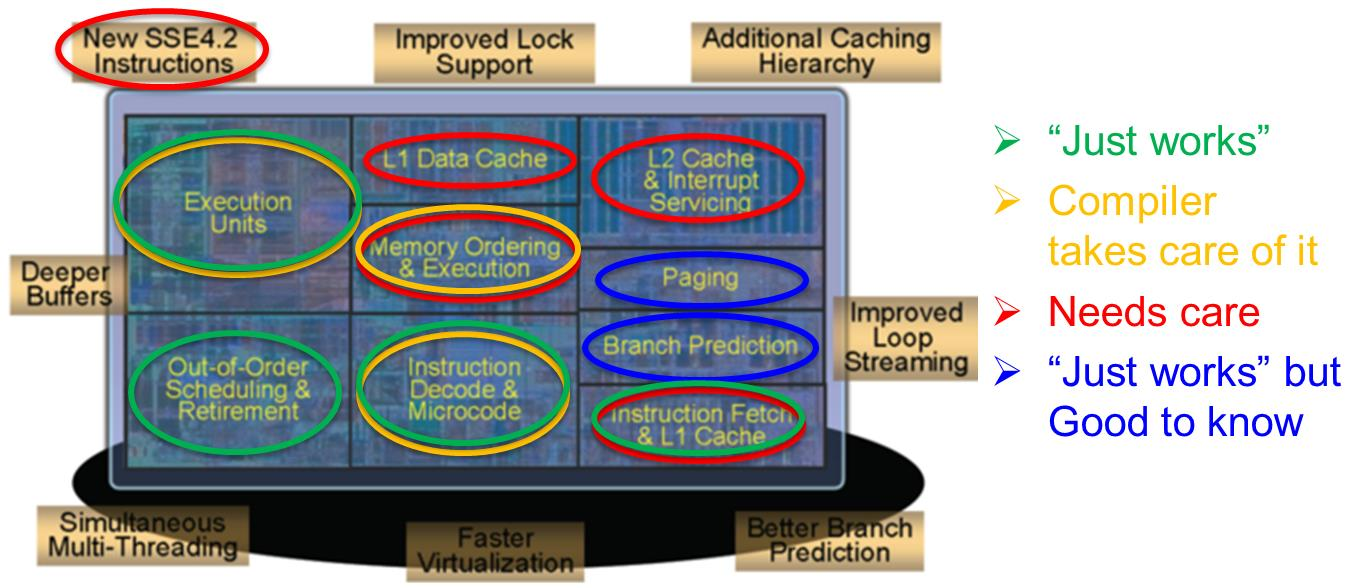
\includegraphics[width=0.9\textwidth]{content/1/chapter3/images/1.jpg}\\
图3.1 - Pentium CPU的模具图像,带有功能区标记(来源:Intel)
\end{center}

图像顶部是主要功能区域。如果是第一次看到这样的图片,最令人吃惊的细节可能是执行单元,也就是做加法、乘法和我们认为是CPU主要功能的部分,实际上甚至不占用四分之一的硅面。剩下的是其他的东西,其目的基本上是使加法和乘法能够有效地工作。并且,处理器有许多具有不同功能的组件。这些组件有一些是独立工作的,开发者无需做什么就可以使用它们。有些需要精心安排机器码,这主要由编译器完成。但是,超过一半的硅面用于组件,这些组件不仅仅是进行优化,还为了获得处理器的最大性能。开发者需要了解它们是如何工作的,它们可以做什么和不可以做什么,以及什么会影响它们的操作效率(积极和消极)。如果需要真正出色的性能,即使使用那些运行良好的部分,也可以从这些组件中受益。

有很多关于处理器架构的书,包括设计师用来提高性能的所使用的硬件技术。这些书可以作为知识的来源,但本书不会再成为这样的书。这里,我们将着重于探索发挥硬件性能的实际方法,我们先从CPU开始。













































